\chapter{Apa yang Dibutuhkan Tumbuhan}\label{ch:g4:what-plants-need}

Dua pot selada air berdiri di ambang jendela yang sama, disemai pada
hari yang sama. Yang satu disiram, yang lain tidak --- dan dalam
seminggu perbedaannya tertulis dengan warna hijau dan kuning. Dengan
pot, \omterm{def:g2:from-seed-to-plant:seed}{biji} dan kesabaran kamu dapat membuat \omterm{def:g1:plants-around-us:plant}{tumbuhannya} sendiri
menjawab pertanyaan bab ini: apa tepatnya yang dibutuhkan sebuah
\omterm{def:g1:plants-around-us:plant}{tumbuhan} untuk hidup dan tumbuh?

\section{Menanyai tumbuhan: uji yang adil}

\begin{method}[Uji yang adil]\label{met:g4:what-plants-need:fairtest}
Untuk mengetahui apakah sebuah \omterm{def:g1:plants-around-us:plant}{tumbuhan} membutuhkan sesuatu --- air,
cahaya, tanah, kehangatan:
\begin{enumerate}
  \item ambil \emph{dua} pot \omterm{def:g1:plants-around-us:plant}{tumbuhan} yang sama, disemai dengan cara
        yang sama;
  \item perlakukan keduanya persis sama dalam segala hal \emph{kecuali
        satu hal yang diuji} --- yang satu mendapatkannya, yang lain
        tidak;
  \item tunggulah beberapa hari atau minggu, lalu bandingkan;
  \item setiap perbedaan pasti datang dari satu hal yang kamu ubah:
        ujinya adil.
\end{enumerate}
Pot yang tidak disentuh disebut \emph{kontrol}\index{kontrol
percobaan}: ia memperlihatkan apa yang terjadi ketika tidak ada yang
hilang.
\end{method}

\begin{example}[Mengapa dua pot dan bukan satu]\label{ex:g4:what-plants-need:control}
Andaikan sebuah pot tunggal yang tidak disiram menjadi layu. Apakah
itu karena air yang hilang --- atau karena udara mendadak dingin, atau
karena \omterm{def:g2:from-seed-to-plant:seed}{bijinya} buruk? Dengan kembarannya yang disiram berdiri hijau di
sebelahnya, ditumbuhkan dari bungkus yang sama di ruangan yang sama,
keraguannya lenyap: kedua kembar itu hanya berbeda dalam hal air.
Percobaan satu pot tidak meyakinkan siapa pun, apalagi seorang ahli
\omterm{def:g1:living-or-not:living}{biologi}.
\end{example}


\begin{omfigure}
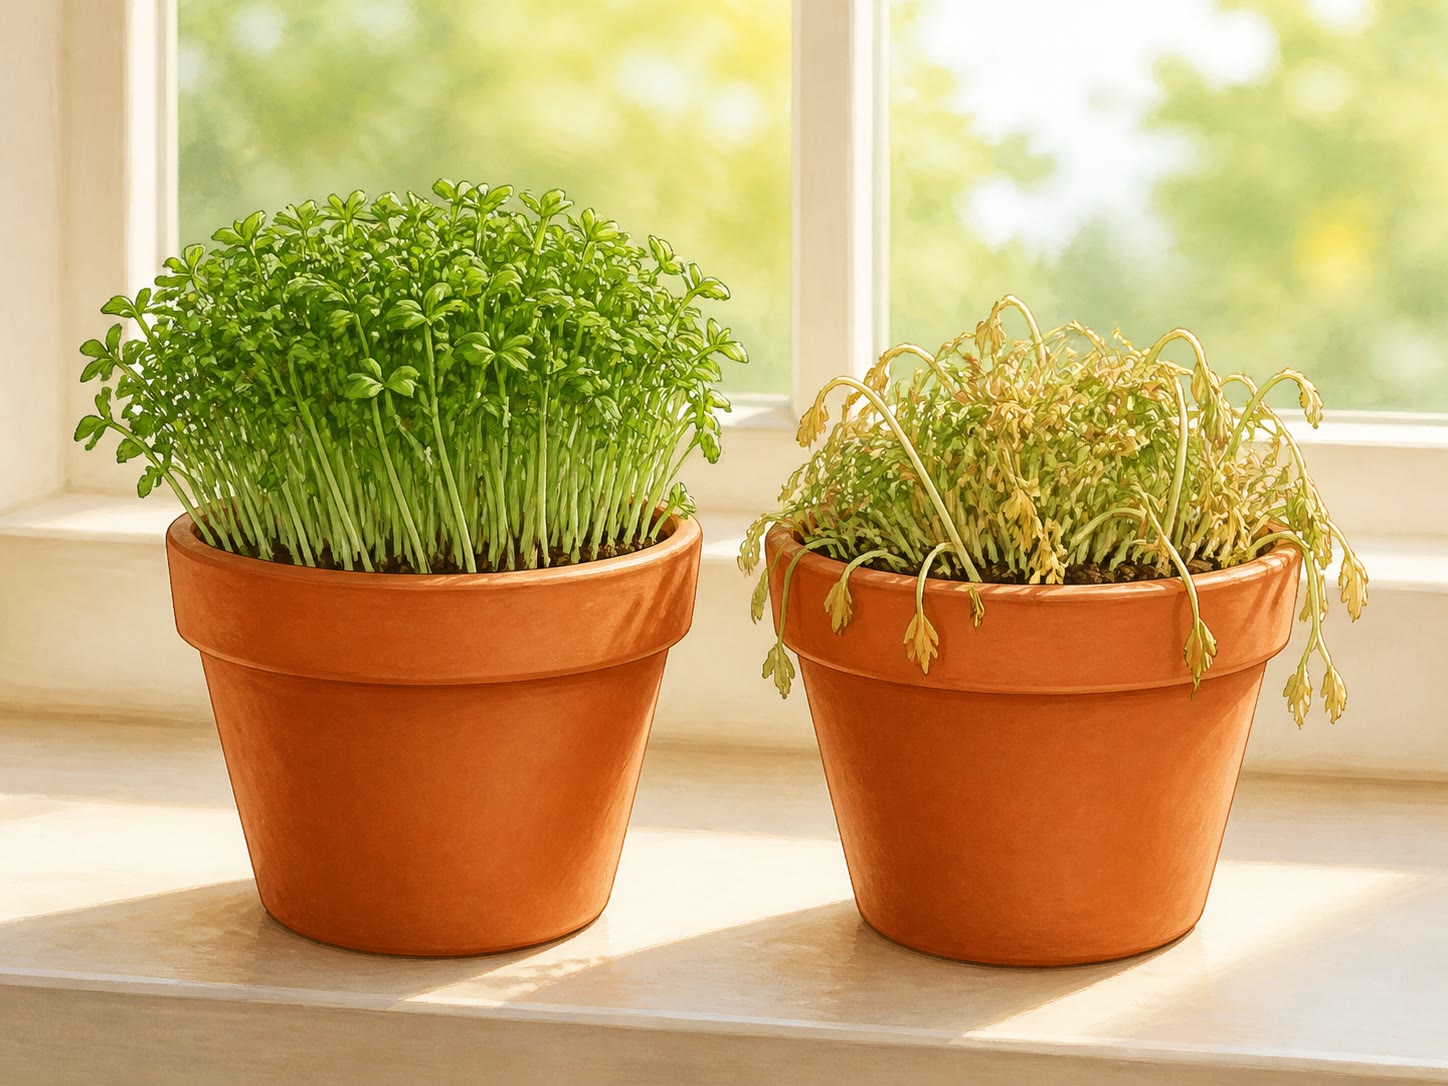
\includegraphics[width=0.58\linewidth]{images/book1/ai/g4-plants-cresspots.jpg}

{\small Percobaan yang sama di ambang jendela sungguhan, sesudah satu
minggu: kedua kembarnya sekarang berbeda dalam segala hal yang
terlihat --- justru karena mereka berbeda dalam satu hal saja.}
\end{omfigure}

\section{Apa yang diungkapkan ujiannya}

\begin{proposition}[Kebutuhan sebuah tumbuhan]\label{prop:g4:what-plants-need:needs}
Uji yang adil, yang dijalankan untuk tiap kebutuhan secara bergiliran,
menunjukkan bahwa sebuah \omterm{def:g1:plants-around-us:plant}{tumbuhan} membutuhkan:
\begin{itemize}
  \item \emph{air} --- pot yang tidak disiram layu lalu mati;
  \item \emph{cahaya} --- pot di dalam lemari tumbuh pucat, memanjang
        dan lemah, lalu menyerah: tanpa cahaya, tidak ada makanan
        \omterm{def:g1:plants-around-us:plant}{tumbuhan} yang dibuat;
  \item \emph{udara} --- kalau ditutup rapat dari udara segar,
        pertumbuhannya berhenti;
  \item \emph{kehangatan} --- dalam keadaan dingin, \omterm{def:g2:from-seed-to-plant:seed}{biji} menunggu
        (\cref{prop:g2:from-seed-to-plant:needs}) dan pertumbuhannya
        membeku sampai berhenti;
  \item \emph{garam mineral}\index{garam mineral}: sejumlah kecil zat
        bergizi yang diminum \omterm{def:g1:plants-around-us:parts}{akarnya} dalam keadaan terlarut di dalam
        air tanah --- di dalam air murni saja, sebuah \omterm{def:g1:plants-around-us:plant}{tumbuhan} segera
        kehabisan.
\end{itemize}
\end{proposition}
\admitted

\begin{example}[Si tawanan yang pucat]\label{ex:g4:what-plants-need:pale}
Uji lemari pada \cref{exo:g1:plants-around-us:8}, yang dijalankan
dengan benar bersama kembaran yang mendapat cahaya, memberi hasil yang
mencolok: si tawanan bukan sekadar murung melainkan \emph{kuning
pucat} --- ia berhenti membuat zat hijaunya --- dan anehnya
\emph{tinggi}, memanjang seolah mencari cahaya yang hilang. Tumbuh
tanpa cahaya berarti membelanjakan tanpa menghasilkan; begitu cadangan
\omterm{def:g2:from-seed-to-plant:seed}{bijinya} terbakar habis, ia berhenti.
\end{example}

\begin{remark}[Mengapa tukang kebun memberi makan tanahnya]\label{rem:g4:what-plants-need:soil}
Kompos dan pupuk kandang bukanlah ``santapan'' \omterm{def:g1:plants-around-us:plant}{tumbuhan} --- \omterm{def:g1:plants-around-us:plant}{tumbuhan}
tidak memakan siapa pun. Keduanya mengisi ulang \omterm{prop:g4:what-plants-need:needs}{garam mineral} tanah,
yang diangkut pergi oleh panen tahun demi tahun. Tempat kompos pada
\cref{ex:g2:caring-for-nature:compost} menutup gelangnya: apa yang
diberikan tanah kepada sayurnya, dikembalikan kulit sayurnya kepada
tanah.
\end{remark}

\section{Apa yang diperbuat tumbuhan dengan yang diambilnya}

\begin{proposition}[Tumbuhan membuat materinya sendiri]\label{prop:g4:what-plants-need:make}
\omterm{def:g1:animals-around-us:animal}{Hewan} tumbuh dengan memakan \omterm{def:g1:living-or-not:living}{makhluk hidup} lain. \omterm{def:g1:plants-around-us:plant}{Tumbuhan} tidak memakan
siapa pun: dengan air dan \omterm{prop:g4:what-plants-need:needs}{garam mineral} dari tanah, udara, dan \omterm{prop:g3:balanced-diet:jobs}{energi}
\emph{cahaya} yang ditangkap \omterm{def:g1:plants-around-us:parts}{daun} hijaunya, ia \emph{membuat materinya
sendiri} --- \omterm{def:g1:plants-around-us:parts}{batang}, \omterm{def:g1:plants-around-us:parts}{daun}, \omterm{def:g1:plants-around-us:parts}{akar} dan \omterm{def:g2:from-seed-to-plant:seed}{biji} yang baru. Itulah sebabnya
cahaya bagi \omterm{def:g1:plants-around-us:plant}{tumbuhan} sama seriusnya dengan makan dan minum, dan
sebabnya \omterm{def:g1:plants-around-us:parts}{daun} hijaunya menghadap ke langit.
\end{proposition}
\admitted

\begin{example}[Sebatang pohon dari hampir tidak ada apa-apa]\label{ex:g4:what-plants-need:tree}
Tanamlah sebutir \omterm{def:g2:from-seed-to-plant:seed}{biji} dalam sebuah pot besar berisi tanah yang sudah
ditimbang, tunggulah bertahun-tahun, dan sebatang pohon kecil berdiri
di situ --- namun tanahnya nyaris tidak kehilangan beratnya. Kayu
pohonnya tidak dikeruk dari potnya: ia \emph{dibuat}, dari air, udara
dan cahaya, di dalam bengkel hijau \omterm{def:g1:plants-around-us:parts}{daunnya}. Dari mana datangnya materi
\omterm{def:g1:living-or-not:living}{makhluk hidup} akan menyibukkan kita lagi pada tahun-tahun berikutnya.
\end{example}

\begin{remark}[Yang hijau menghidupi semua orang]\label{rem:g4:what-plants-need:everyone}
Ingatlah \cref{prop:g3:food-chains:start}: setiap \omterm{def:g3:food-chains:chain}{rantai makanan}
bermula pada \omterm{def:g1:plants-around-us:plant}{tumbuhan}. Sekarang kita melihat mengapa hal itu memang
harus begitu --- \omterm{def:g1:plants-around-us:plant}{tumbuhan} adalah satu-satunya mata rantai yang membuat
materi baru dari bahan yang tak hidup. Setiap suapan yang dimakan
siapa pun, di mana pun, dibuat lebih dahulu di dalam sehelai \omterm{def:g1:plants-around-us:parts}{daun}.
\end{remark}

\section{Latihan}

\begin{exercise}[$\star$]\label{exo:g4:what-plants-need:1}
Sebutkan kelima kebutuhan sebuah \omterm{def:g1:plants-around-us:plant}{tumbuhan}.
\end{exercise}

\begin{exercise}[$\star$]\label{exo:g4:what-plants-need:2}
Dalam sebuah uji yang adil, berapa banyak hal yang boleh berbeda
antara kedua potnya? Pot yang tidak disentuh disebut apa?
\end{exercise}

\begin{exercise}[$\star$]\label{exo:g4:what-plants-need:3}
Lukiskan rupa sebuah \omterm{def:g1:plants-around-us:plant}{tumbuhan} yang ditumbuhkan dua minggu dalam gelap.
Kebutuhan mana yang hilang, dan apa yang tidak dapat dibuatnya?
\end{exercise}

\begin{exercise}[$\star$]\label{exo:g4:what-plants-need:4}
Apa itu \omterm{prop:g4:what-plants-need:needs}{garam mineral}, dan bagaimana \omterm{def:g1:plants-around-us:plant}{tumbuhannya} memasukkannya?
\end{exercise}

\begin{exercise}[$\star$]\label{exo:g4:what-plants-need:5}
Mengapa tukang kebun menebarkan kompos, kalau \omterm{def:g1:plants-around-us:plant}{tumbuhan} tidak makan?
\end{exercise}

\begin{exercise}[$\star$]\label{exo:g4:what-plants-need:6}
Bagaimana cara tumbuh sebuah \omterm{def:g1:plants-around-us:plant}{tumbuhan} berbeda dari cara tumbuh seekor
\omterm{def:g1:animals-around-us:animal}{hewan}, menurut \cref{prop:g4:what-plants-need:make}?
\end{exercise}

\begin{exercise}[$\star$]\label{exo:g4:what-plants-need:7}
Pada \cref{ex:g4:what-plants-need:tree}, tanah di dalam potnya nyaris
tidak kehilangan berat sementara pohonnya tumbuh. Dari mana datangnya
materi pohonnya?
\end{exercise}

\begin{exercise}[$\star$]\label{exo:g4:what-plants-need:8}
Cobalah: rancang lalu jalankan uji adil tentang air pada gambarnya
dengan selada air --- dua pot, satu perbedaan. Catat apa yang kamu
lihat sesudah seminggu.
\end{exercise}

\begin{exercise}[$\star\star$]\label{exo:g4:what-plants-need:9}
Lucas ``membuktikan'' bahwa \omterm{def:g1:plants-around-us:plant}{tumbuhan} membutuhkan musik: ia bernyanyi
kepada satu pot selama sebulan, dan pot itu tumbuh subur. Apa yang
hilang dari percobaannya, menurut
\cref{met:g4:what-plants-need:fairtest}? Rancanglah versi yang
sungguh-sungguh mengujinya.
\end{exercise}

\begin{exercise}[$\star\star$]\label{exo:g4:what-plants-need:10}
Sebuah \omterm{def:g1:plants-around-us:plant}{tumbuhan} air tumbuh terendam sepenuhnya, tanpa \omterm{def:g1:plants-around-us:parts}{akar}, namun
sehat. Kebutuhan mana di antara kelimanya yang jelas masih
dipenuhinya, dan bagaimana --- dan kebutuhan mana yang disediakan
airnya sebagai ganti tanah?
\end{exercise}

\begin{exercise}[$\star\star\star$]\label{exo:g4:what-plants-need:11}
Dua pot \omterm{def:g1:plants-around-us:parts}{daun} mint yang serupa: yang satu dalam pasir dengan air hujan
murni, yang lain dalam tanah kebun, keduanya disiram dan disinari
sama. Sesudah dua bulan pot pasirnya kecil dan menguning. Kebutuhan
mana yang dipisahkan uji adil ini --- dan mengapa \omterm{def:g1:plants-around-us:plant}{tumbuhan} pasirnya
sempat tumbuh sama sekali pada mulanya?
\end{exercise}
